\documentclass[twocolumn]{article}

\usepackage[utf8]{inputenc}

\usepackage{amsmath}
\usepackage{graphicx}
\usepackage{titling}

\usepackage{stfloats}

\pretitle{\begin{center}\Huge\bfseries}
\posttitle{\par\end{center}\vskip 0.5em}
\preauthor{\begin{center}\Large\ttfamily}
\postauthor{\end{center}}
\predate{\par\large\centering}
\postdate{\par}

%******************************
\usepackage[T1]{fontenc}

\usepackage[tracking]{microtype}

\usepackage[sc,osf]{mathpazo}   % With old-style figures and real smallcaps.
\linespread{1.025}              % Palatino leads a little more leading

% Euler for math and numbers
\usepackage[euler-digits,small]{eulervm}
\AtBeginDocument{\renewcommand{\hbar}{\hslash}}

\usepackage{ntheorem}

% No easy way of putting the theorem description in italics?
% It seems I need to define a new style...
\makeatletter
\newtheoremstyle{mystyle}% 
   {\item[\hskip\labelsep \theorem@headerfont ##1\ ##2\theorem@separator]}% 
   {\item[\hskip\labelsep \theorem@headerfont ##1\ ##2\ \textit{(##3)}\theorem@separator]}
\makeatother
\theoremstyle{mystyle}
\theoremheaderfont{\scshape}
\theorembodyfont{\upshape}

\newtheorem{theorem}{theorem}
\usepackage{listings}


%* \usepackage{biblatex}

%* \addbibresource{library.bib}

% *** CITATION PACKAGES ***
\usepackage{natbib}
\bibliographystyle{unsrtnat}
\usepackage{uri}

\usepackage{tcolorbox}
\tcbuselibrary{minted,breakable,xparse,skins}

\definecolor{bg}{gray}{0.95}
\DeclareTCBListing{mintedbox}{O{}m!O{}}{%
  breakable=true,
  listing engine=minted,
  listing only,
  minted language=#2,
  minted style=default,
  minted options={%
    linenos,
    gobble=0,
    breaklines=true,
    breakafter=(,
    fontsize=\footnotesize, %* \small
    numbersep=8pt,
    #1},
  boxsep=0pt,
  left skip=0pt,
  right skip=0pt,
  left=25pt,
  right=0pt,
  top=3pt,
  bottom=3pt,
  arc=5pt,
  leftrule=0pt,
  rightrule=0pt,
  bottomrule=2pt,
  toprule=2pt,
  colback=bg,
  colframe=orange!70,
  enhanced,
  overlay={%
    \begin{tcbclipinterior}
    \fill[orange!20!white] (frame.south west) rectangle ([xshift=20pt]frame.north west);
    \end{tcbclipinterior}},
  #3
}
  
\usepackage{xcolor}
\usepackage{soul}

\definecolor{Light}{gray}{.90}
\sethlcolor{Light}
\let\OldTexttt\texttt
\renewcommand{\texttt}[1]{\OldTexttt{\hl{#1}}}
\setlength{\parindent}{0pt}

\title{Multifunctionality in Recurrent neural networks based on LSTMs}
\author{Ian Emerik Leko}
\date{September 2022}

\begin{document}

\lstset{
  basicstyle=\ttfamily,
  columns=fullflexible,
  keepspaces=true,
}


\twocolumn[
  \begin{@twocolumnfalse}
  \maketitle
  
  \vspace{5pt}
  
\section*{Declaration of Authorship} 
This is to certify that the work I am submitting is my own and has not been submitted for another degree, either at University College Cork or elsewhere. All external references and sources are clearly acknowledged and identified within the contents. I have read and understood the regulations of University College Cork concerning plagiarism and intellectual property.

\section*{Acknowledgements}
I would first like to thank both of my supervisors Andrew Keane and Brendan Byrne who's input and guidance and input have been invaluable thought this project. I would also like to thank Brendan for the resources and data provided through TOMRA as this project would not have been possible without it. A special thanks goes to Jim Henry and Kate O'Byrne at TOMRA who have been great helps and fantastic resources while trying to understand the data and systems. A final gratitude goes to my family who have supported me throughout the MSc program.
 
\section*{Summary}

Biological neural networks are inherently multifunctional - they can exhibit multiple patterns based on the needs of the environment. In this thesis, we ask ourselves whether we can replicate such behaviour using the LSTM neural networks. Previous work has been established that this effect can be observed in Reservoir Computers, and we extend these results to LSTMs.

\textbf{Keywords}: Long-Short Term Memory; Neural Networks; Dynamical Systems; Limit Cycle

In this report we will do the following
\begin{enumerate}
    \item Briefly describe the motivation behind the multifunctionality
    \item Review the previous work done with Reservoir Computers
    \item Explain LSTMs in depth
    \item Review modelling of dynamical systems with LSTMs
    \item Finally, explore multifunctionality using LSTMs
\end{enumerate}
  \end{@twocolumnfalse}
]

\twocolumn[
  \begin{@twocolumnfalse}
  \begin{center}
       \section*{PART I - Introduction}
  \end{center}
  \end{@twocolumnfalse}
]

\section*{Motivation}

In this section we will describe the concept of multifunctionality and the relevance to the audience.

\subsection*{Biological Perspective of Neural Networks}
``A basic tenet of neuroscience is that the ability of the brain to produce complex behaviors such as sensory perception or motor control arises from the interconnection of neurons into networks or circuits.`` \cite{gettingEmergingPrinciplesGoverning1989}. 
Such networks have been a source of inspiration for \textit{artificial neural networks} (ANN). Similarly to a biological neuron, which ``\dots receives multiple signals through the synapses contacting its dendrites and sends a single stream of action potentials out through its axon\dots'', \cite{kriegeskorteNeuralNetworkModels2019}, an \textit{artifical neuron} is a unit that combines multiple inputs and provides a single discernible output. Such units can be combined in networks of arbitrary design. 
A sketch of a basic ANN is shown in Figure \ref{fig:neutral-network-diagram}.
\begin{figure}[!b]
    \begin{center}
    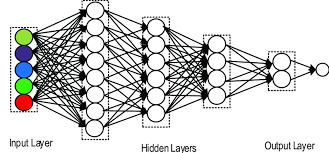
\includegraphics[scale=0.5]{Images/neutral-network-diagram.png}
    \caption{Sketch of an ANN with hidden layers, \cite{dumorEstimatingChinaTrade2019}}
    \label{fig:neutral-network-diagram}
    \end{center}
\end{figure}
Each layer's units connect to each of the next layer's units, and units themselves first calculate the linear combination of the inputs, and then perform a non-linear \textit{activation} on that linear combination. A network of this model, with at least one \textit{hidden} layer - i.e. a layer in between input and ouput layers, can be shown to be a \textit{universal approximator}, i.e. an algorithm that can approximate arbitrary functions, \cite{scarselliUniversalApproximationUsing1998}.

\subsection*{Biological Perspective of Multifunctionality}
We will follow \cite{flynnMultifunctionalityReservoirComputer2021a} in defining the multifunctionality as the networks ``...  of neurons whose activity patterns can change on the demand of performing a given duty, but synapses remain fixed.'' In other words, a multifunctional network can perform multiple tasks, without changing its inner structure. Such a definition is biologically motivated: even intuitively, we have a single brain which can both, say, write a poem and drive a bike. To be more specific, for example, \cite{briggmanImagingDedicatedMultifunctional2006} examined the neural activation of a medicinal leach when either crawling or swimming. The key finding was that the motions are driven both by multifunctional and dedicated circuitry. Even more interestingly, the overlap between neurons for the two motions is great: 93\% of the neurons that activated when swimming also activated when crawling. One of the proposed explanations is that ``...a single network driven at two different frequencies could generate motor patterns with different phase relationships without recruiting any additional neurons.'' (\cite{briggmanImagingDedicatedMultifunctional2006}). Furthermore, \cite{eschEvidenceSequentialDecision2002} showed that this switch in the behaviour happens according to the external stimuli, in this case the salinity level.

\newpage

\twocolumn[
  \begin{@twocolumnfalse}
  \begin{center}
       \section*{PART II - Long-Short Term Memory Neural Networks}
  \end{center}
  \end{@twocolumnfalse}
]

\section*{Introduction}

We assume the reader is familiar with the concept of neural networks and the intricancies of ANNs (i.e. the vanilla NNs). In this part we will first introduce and describe recurrent neural networks (RNNs) as following:
\begin{enumerate}
    \item Motivate development of recurrent neural networks (RNNs)
    \item Mathematically describe basic RNNs
    \item Motivate development of long-short term memory neural networks (LSTMs)
    \item Mathematically describe LSTMs
\end{enumerate}
Then, we will describe the computational representation of such networks via \textit{computational graphs} in the following order:
\begin{enumerate}
    \item Introduce the idea of computational graphs, forward- \& backward-propagation
    \item Represent RNNs as a computational graph
    \item Represent LSTMs as a computational graph
\end{enumerate}

Finally, we will explore LSTM impementation in \texttt{Tensorflow 2.0} and \texttt{Keras} packages. This will serve as the foundation for the further talk on multifunctionality in LSTMs.

\subsection*{Recurrent Neural Networks}
\subsubsection*{Motivation}
ANNs, while universal function approximators, do not take into account relationship between inputs, most notably the temporal relationship. For example and following \cite{aggarwalNeuralNetworksDeep2018}, suppose we were to pass the sentences
\begin{align}
    &\texttt{The cat chased the mouse}\\
    &\texttt{The mouse chased the cat}
\end{align}
to an ANN. Each word would be an input and the network would think of the two sentences as being the same. However fine this might be for a simpler task such as classification, it is missing the nuance required for more complicated tasks such as machine translation. Thus for more complicated tasks when working with sequential data, we want to encapsculate that sequentiallity in our model.

\subsubsection*{History}
Recurrent neural networks, as in the neural networks with feedback/self-looping structure have been present in the reasearch since 1980s, for example in \cite{rumelhartLearningInternalRepresentations1985} and \cite{jordanSerialOrderParallel1986} which investigated network structures suitable for sequential data, especially using the recurrent links to provide the network with dynamic memory. Then \cite{elmanFindingStructureTime1990} published the seminal \textit{Finiding Structure in Time} which provided for a reference RNN model for the time to come. In the next section we will describe the \textit{Elman} model mathematically.

\subsubsection*{Mathematics}
For this section we will describe how a classic, or Elman, RNN operates. Diagram of such an RNN is shown in figure \ref{fig:rnn-diagram-temporal}. The network has a inner variable, the \textit{hidden state}, denoted by $h_0$. Usually it is initialised to a vector of $0$s. Then it is successively combined with inputs $x_1,\dots,x_n$ to obtain a new hidden state. Finally, each hidden state can produce an output of its own. Sometimes this is useful, but sometimes we only care about the final output after we have run through all the inputs (for example, in case of classification).

Mathematically, we start with variables
$$ h_0,\quad x_1, \quad \dots, \quad x_n $$
each representing a vector in $\mathbb{R}^d$ for some arbitrary dimension $d$. Then, at each time step $t$ correspoding to the input $x_t$ we can calculate the new hidden state $h_t$ and the correspoding output $y_t$ as

\begin{align}
    h_t &= \sigma\left(W_{xh}x_t + W_{hh}h_{t-1}\right) \\
    y_t &= W_{hy}h_t
\end{align}

where

$$ W_{xh}, \quad W_{hh}, \quad W_{hy} $$

are inner parameter matrices that are learnable. $\sigma$ represents an arbitrary non-linear activation function.

\begin{figure*}[!b]
    \begin{center}
        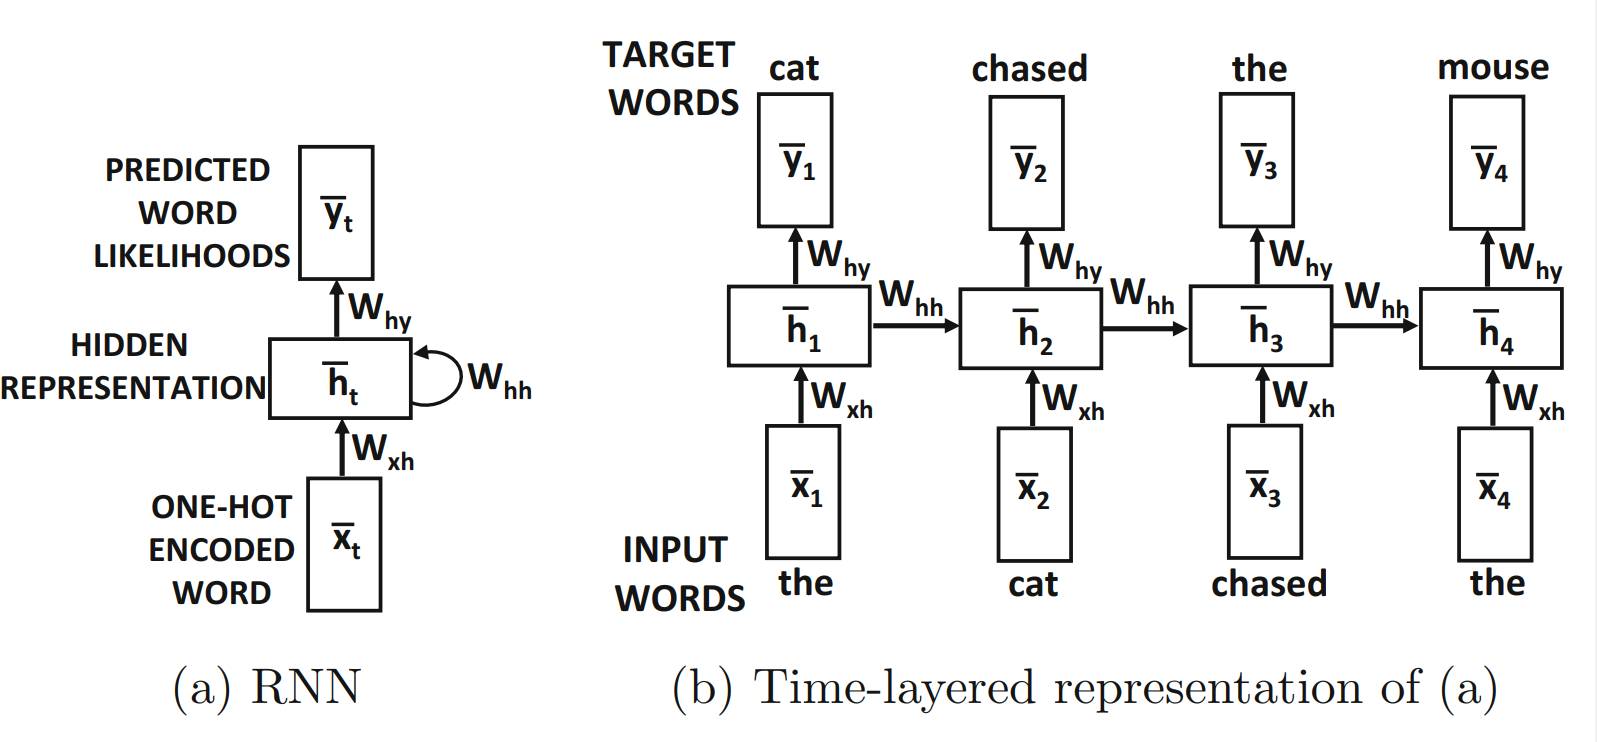
\includegraphics[scale=0.4]{Images/rnn-diagram-temporal.png}
        \caption{RNN and its temporal representation (\cite{aggarwalNeuralNetworksDeep2018})}
        \label{fig:rnn-diagram-temporal}
    \end{center}
\end{figure*}

\subsection*{Long Short Term Memory}
\subsubsection*{Motivation \& History}
RNNs have been notorious for being hard to train, especially over long sequences with the standard backpropagation techniques for learning: \cite{bengioLearningLongtermDependencies1994} provide detailed overview of the problem and rudimentary solutions.Usually the problems crystalise in one of the two ways: gradient vanishing and gradient exploding (see Chapter 7 of \cite{aggarwalNeuralNetworksDeep2018} for an overview). Multiple solutions have been proposed, but the most popular one has been the Long Short Term Memory variant introduced by \cite{hochreiterLongShortTermMemory1997}. In fact, ``Almost all exciting results based on RNNs have been achieved by LSTM, and thus it has become the focus of deep learning.'' (\cite{yuReviewRecurrentNeural2019}). The ``vanilla'' LSTM we will describe in detail in the following sections is assumed to be the original LSTM with addition of forget gate and with peephole connections (\cite{vanhoudtReviewLongShortTerm2020}). This format has been the upgrade of the original model by one of the inventors in \cite{gersLearningForgetContinual2000}. The 

\subsubsection*{Mathematics}
Figure \ref{fig:lstm-architecture} shows diagram of a vanilla LSTM block. Note that, compared with Elman RNN, we have one more hidden variable, denoted by $c$ (cell state). The key innovation of LSTM is that we control information flow to-and-from the cell state with carefully devised operations.

Again we start with inner states and the input variables
$$ c_0, \quad h_0, \quad x_1, \quad \dots, \quad x_n $$
where 
$$c_0\in\mathbb{R}^C,\ h_0\in\mathbb{R}^H, \textrm{ and } x_i\in\mathbb{R}^X\ \forall i\in\{1,\dots,n\}$$
Following \cite{yuReviewRecurrentNeural2019}, the formulas for the gates and the hidden states at the time step $t$, corresponding to the input $x_t$, are:
\begin{align}
    f_t &= \sigma\left( W_{fh}h_{t-1} + W_{fx}x_t + P_f \odot c_{t-1} + b_f \right) \\
    i_t &= \sigma\left( W_{ih}h_{t-1} + W_{ix}x_t + P_i \odot c_{t-1} + b_i \right) \\
    \tilde{c}_t &= \tanh\left( W_{\tilde{c}h}h_{t-1} + W_{\tilde{c}x}x_t + b_{\tilde{c}} \right) \\
    c_t &= f_t \odot c_{t-1} + i_t \odot \tilde{c}_t \\
    o_t &= \sigma\left( W_{oh}h_{t-1} + W_{ox}x_t + P_o \odot c_t + b_o \right) \\
    h_t &= o_t \odot \tanh(c_t)
\end{align}

\begin{figure*}[!b]
    \begin{center}
        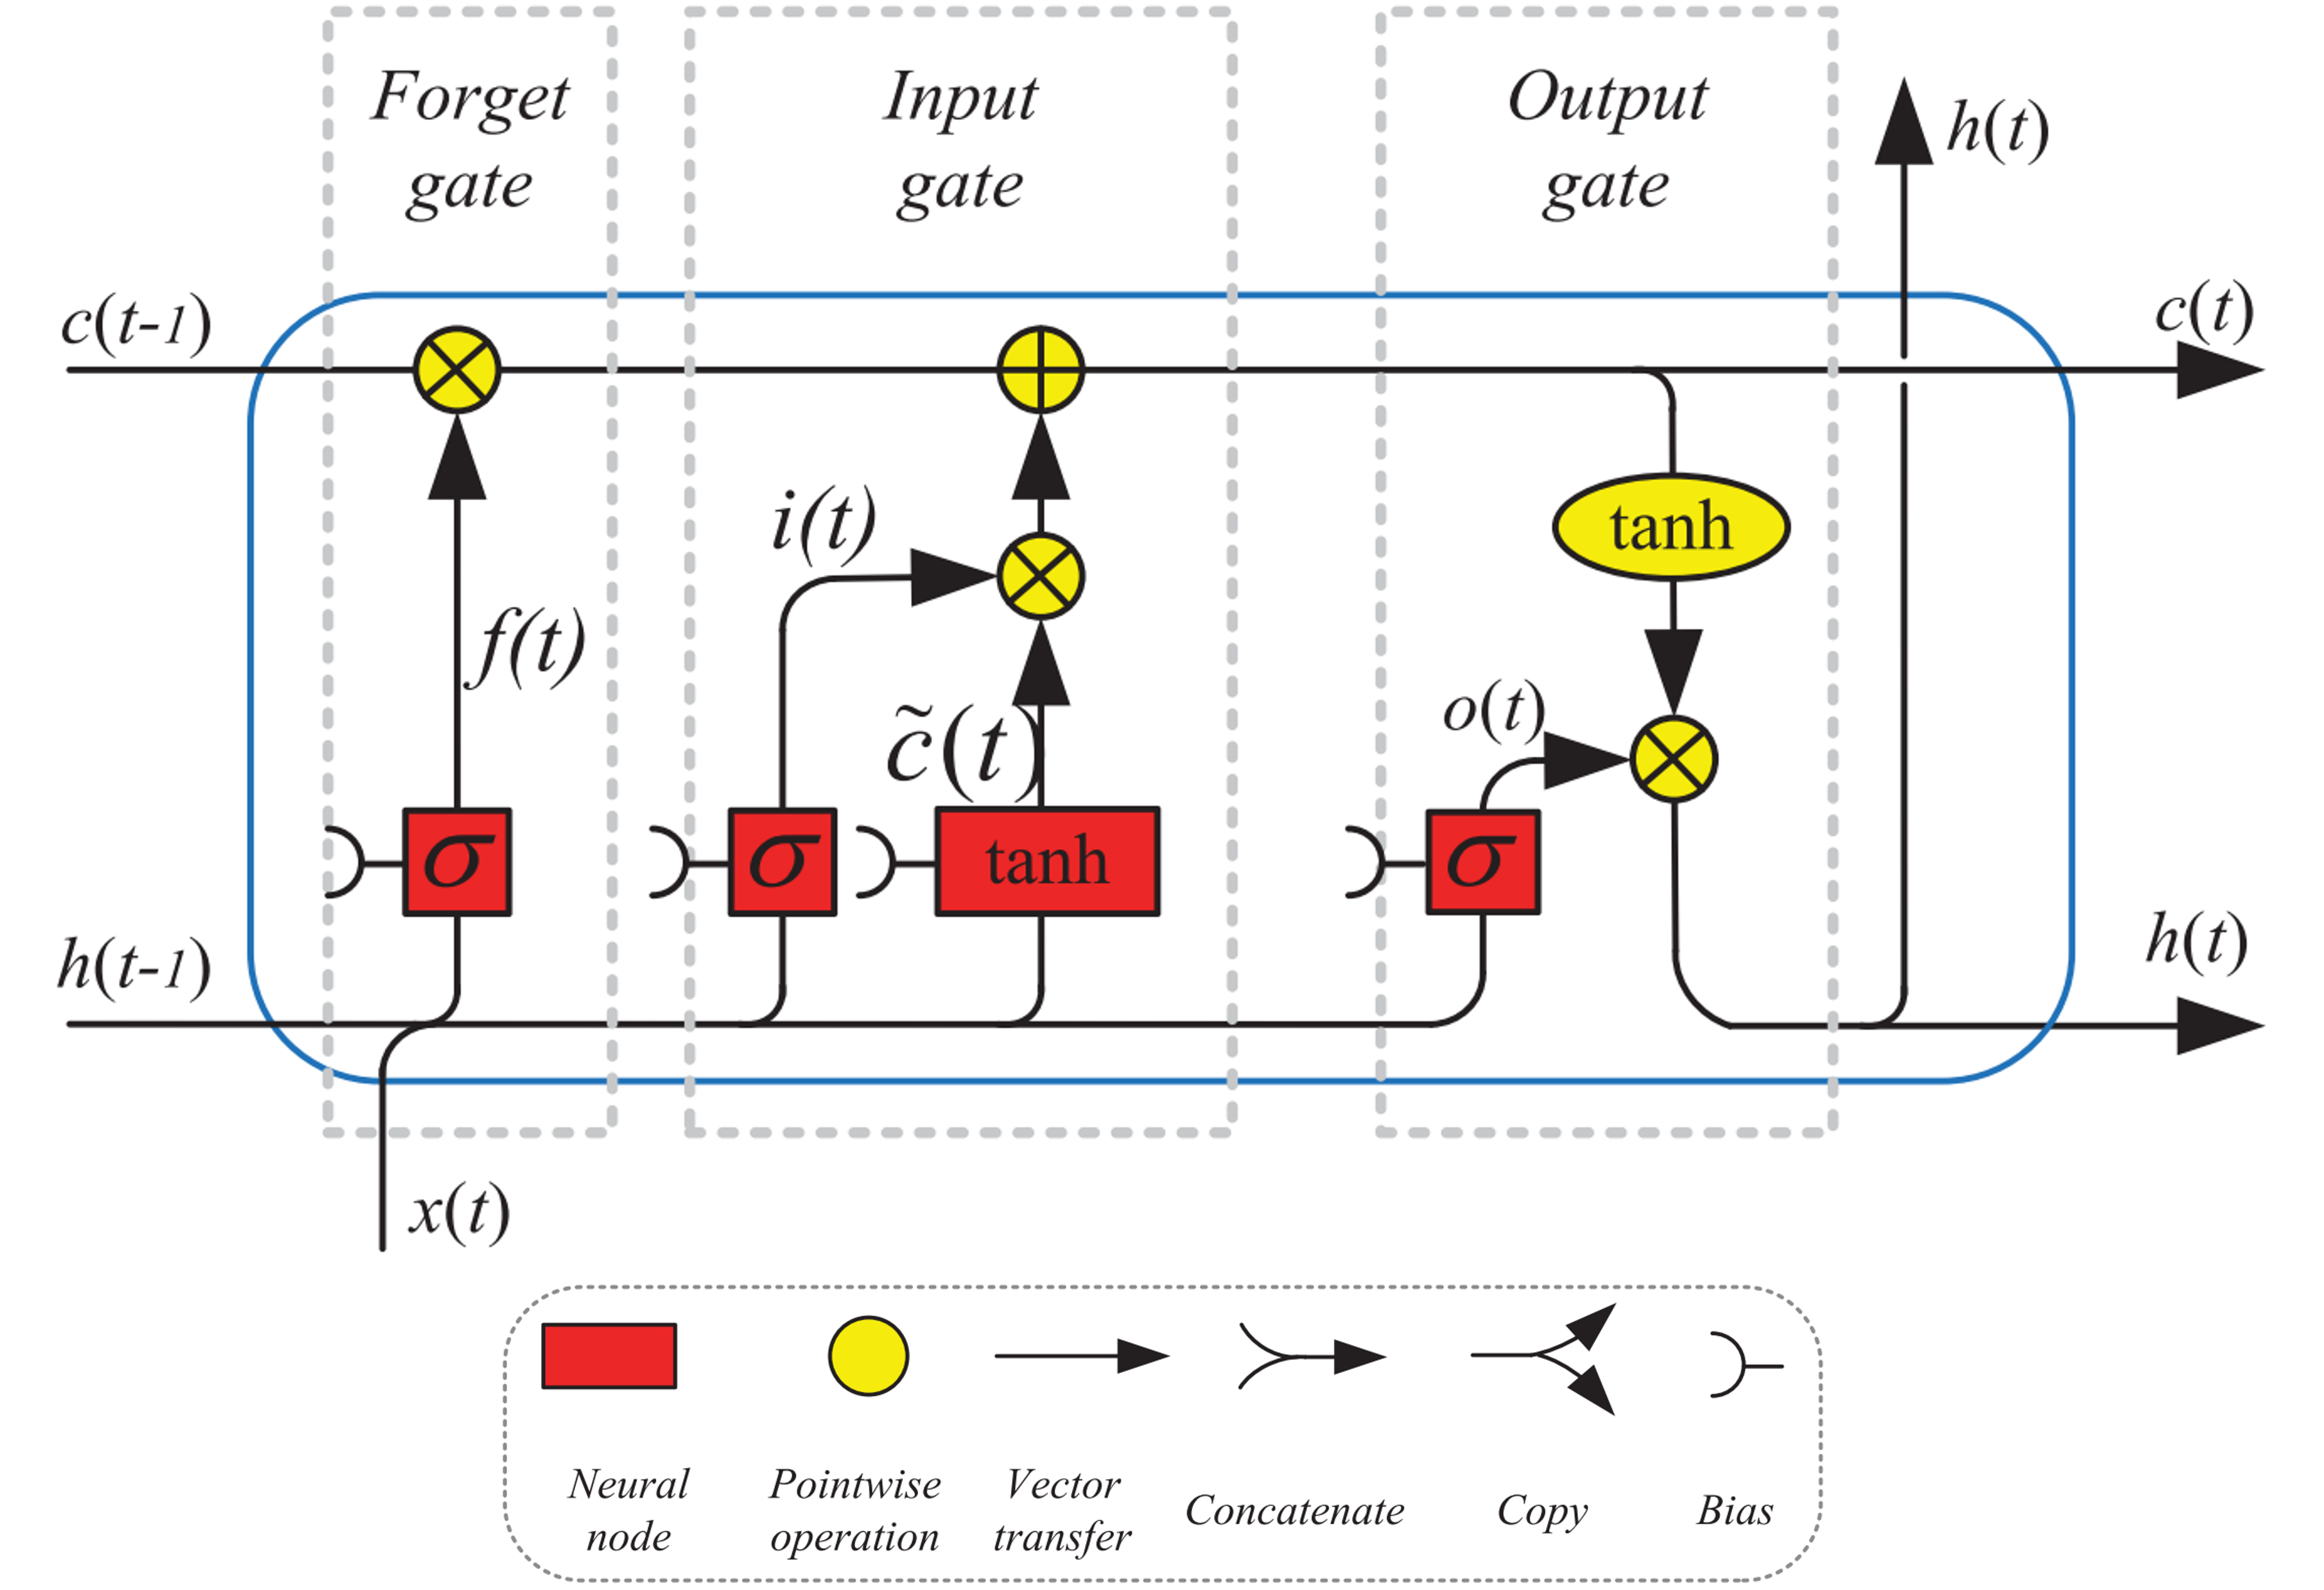
\includegraphics[scale=0.55]{Images/lstm-architecture.png}
        \caption{Vanilla LSTM cell (\cite{yuReviewRecurrentNeural2019})}
        \label{fig:lstm-architecture}
    \end{center}
\end{figure*}

where the $\odot$ represents the Hadamard product (the element-wise multiplication). Now we have 
$$ P_f, \quad P_i, \quad P_o $$
as the peephole weights for the forget, input and the output gate respectively. Similarly to before, 
$$ W_{fh}, \quad W_{fx}, \quad W_{ih}, \quad W_{ix}, \quad W_{\tilde{c}h}, \quad W_{\tilde{c}x}, \quad W_{oh}, \quad W_{ox} $$
are the trainable inner matrices and
$$ b_f, \quad b_i, \quad b_{\tilde{c}}, \quad b_o $$
represent the trainable biases.

\newpage
\subsection*{LSTMs in \texttt{tensorflow}}
In this section we describe how the LSTMs are implemented as part of the \textit{Tensorflow 2.0} and \textit{Keras} libraries for the Python programming language. We will discuss how the parameters correspond to the mathematics discussed in the previous sections.

\subsubsection*{Tensorflow 2.0 \& Keras}
``TensorFlow is an interface for expressing machine learning algorithms and an implementation for executing such algorithms.'' (\cite{abadiTensorFlowLargeScaleMachine}). On top of \texttt{tensorflow}, Keras (\cite{chollet2015keras}) provides top-line functionality for quick creation and maintainance of commonly used neural network types, including LSTMs. Let us look at the parameters for the \texttt{keras} implementation (whole list is shown in Figure \ref{fig:keras-LSTM-parameters}). LSTM is incorporated directly in \texttt{keras} as a layer found in \texttt{tensorflow.keras.layers.LSTM} as seen in the Figure \ref{fig:keras-LSTM-parameters}.

\begin{enumerate}
    \item \texttt{units} - number of separate LSTM networks that the layer models. It is one of the dimensions of the output
    \item \texttt{activation} - 
\end{enumerate}

\begin{figure}
    \begin{center}
        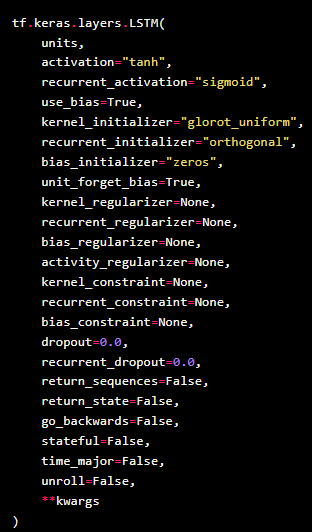
\includegraphics[scale=1]{Images/keras-lstm-parameters.png}
        \caption{Keras LSTM class parameters (\cite{teamKerasDocumentationLSTM})}
        \label{fig:keras-LSTM-parameters}
    \end{center}
\end{figure}




\newpage

\twocolumn[
  \begin{@twocolumnfalse}
  \begin{center}
       \section*{PART III - Basics of Dynamical Systems}
  \end{center}
  \end{@twocolumnfalse}
]

\section*{Introduction}

\newpage

\twocolumn[
  \begin{@twocolumnfalse}
  \begin{center}
       \section*{PART IV - Modelling Dynamical Systems using LSTMs}
  \end{center}
  \end{@twocolumnfalse}
]

\section*{Introduction}

\newpage

\twocolumn[
  \begin{@twocolumnfalse}
  \begin{center}
       \section*{Bibliography}
  \end{center}
  \end{@twocolumnfalse}
]
\bibliography{References/refs}

\end{document}